\documentclass[emulatestandardclasses]{scrartcl}
\usepackage{graphicx}
\usepackage{color}
\usepackage[ngerman]{babel}
\usepackage{hyperref}
\usepackage{fullpage}
\usepackage{calc} 
\usepackage{enumitem}
\usepackage{titlesec}
\newcommand{\todo}[1]{\textcolor{red}{TODO: #1}\PackageWarning{TODO:}{#1!}}
\date{\vspace{-3ex}}
\begin{document}

\title{
	\includegraphics*[width=0.75\textwidth]{ErstesSem/images/hu_logo.png}\\
	\vspace{24pt}
	Hegels Theorie der Weltgeschichte}
\subtitle{Proseminar SS 18\\
          Dr. Dimitris Karydas\\
          Theologische Fakult"at \\ 
          Humboldt Universit"at zu Berlin}
\author{Lennard Wolf\\
        \small{\href{mailto:lennard.wolf@student.hu-berlin.de}{lennard.wolf@student.hu-berlin.de}}}
\maketitle
\begin{abstract}

Hegels Konzept von Weltgeschichte als Fortschritt im Bewusstsein der Freiheit wird im Zusammenhang des Systems des Geistes erläutert. Dem liegt ein Begriff der Geschichtlichkeit zugrunde, der so originär wie bis heute umstritten ist. Die zentralen damit verbundenen Konzepte und Motive von der Vernunft in der Geschichte, der Verwirklichung der Freiheit oder vom Ende der Geschichte werden im Mittelpunkt der Diskussion stehen. Die für Hegels Auffassung von Geschichte ausschlaggebenden Passagen aus den Vorlesungen über die Philosophie der Weltgeschichte, der Enzyklopädie und der Rechtsphilosophie werden gelesen, die auf moodle bereitgestellt werden.
\end{abstract}
\newpage

\tableofcontents
\listoffigures
\newpage


\section{Subjektiver und Objektiver Geist\\(24.04.18)}

\subsection{Organisatorisches}

\begin{itemize}
  \item Moodle-PW: history (ab 27.04.)
  \item Abgabe: Essay/Protokolle zu insgesamt 10 Seiten
  \item F"ur schein der Teilnahme ist ein Referat/ Protokoll abzugeben
  \item Vortrag am 08.05. Enz. 545 - 552
\end{itemize}

\subsection{Einf"uhrung}

\begin{itemize}
  \item Geist ist geschichtlich
  \item was wir sind wsind wir geschichtlich geworden
  \item Der Löwe versteht sich als Löwe (indem er sich als Löwe verhält ("`an sich"'), nicht reflektierend ("`für sich"')), ohne Bewusstsein zu haben
  \item Metareflektion darüber, wie der Mensch sich auf die Natur beziehen kann
  \item Reduplikation der Weltgeschichte anhand des Begriffs
  \item Subjektivität ist zweierlei: das Wesen des Subjekts (vom Subjekt ist erst in der Moderne zu reden; Das Bewusstsein dass alle \emph{rechtlich} frei sind etc. ist ein modernes) und Reflektion
  \item Die Tiere verhalten sich gesellschaftlich, nur sie reflektieren nicht darüber (Karydas: Hegel ist mit Darwin )
  \item Die Natur hat keine \emph{Geschichte} (was nicht heißt, dass sie keine Historie hat)
  \item Unterschied Historie Geschichte: Wird noch besprochen
  \item Feuerbachs Kernbegriff ist die "`Gattung"'
  \item Empfehlung: Tierphilosophie Hegels
  \item Die Idee: Der Algorithmus der Welt, was die Welt z
  \item Begriffe wie "`Idee"', "`Absolutes"' etc. wurden leider früher immer fetischisiert, doch sie sind auf die Welt zurückzuholen, sie sind ganz naiv, konkret gemeint
  \item die Bewegung vom Abstrakten zum Konkreten ist nach oben gerichtet (erste Negation?)
  \item es spielt das partikulare des Konkreten für das Allgemeine keine Rolle
  \item Der Geist ist das sich von Sich-von-sich-selbst-unterscheiden
  \item Bedürfnis zur Philosophie kommt aus dem Bedürfnis zu Begreifen
  \item der konkrete Geist ist die abstrakte Natur
  \item Der Sohn ist die Natur, die Idee ist der alte Mann
  \item  481: Meint gezeigt zu haben, dass der subjektive Geist ist durch die Form des Allgemeinen vermittelt
\end{itemize}


\section{Eigene Notizen}

\begin{itemize}
  \item Subjektiver Geist: Der Mensch als geistige Struktur (Psychologie (Kants Vermögen), Phänomenologie)
  \item Objektiver Geist: Menschliches Miteinander
  \item Absoluter Geist: Wissen des Göttlichen
  \item Bei Hegel ist Sittlichkeit bestimmt als "`Reihe von Pflichten, die wir haben, und die besagt, daß eine auf der Idee gegründete Gesellschaft gefördert und erhalten werden muß"'
  \item Der Staat ist dadurch ausgezeichnet, dass er als Ganzes alle Momente des menschlichen Lebens beinhaltet (familiäres, ökonomisches, politische Institutionen) und sich in seiner Entwicklung auf sich selbst bezieht (ebd.: 330, § 536). Der Staat ist dabei die höchste Weise der Vermittlung von Individualität und Gesellschaftlichkeit, und begründet, beinhaltet und umfasst die familiären und die ökonomischen Beziehungen der Menschen. 
  \item Vernunft ist schon immer da, sie muss nur immer weiter verwirklicht werden
\end{itemize}

\section{Ideen zu Hausarbeit}

\begin{itemize}
  \item Es ist keine Whig history, da nicht gesagt ist, dass der Geist zwangsläufig die Freiheit erlangt, es ist vielmehr einfach eine Sache der Zeit
  \item Indem der Fokus auf den subjektiven Geist zurückgelenkt wird, die Sittlichkeit als schädigend für den subjektiven Geist aberkannt wird und der objektive Geist zum Werkzeug für die erfüllung des subjektiven Willens umgekehrt wird, befinden wir uns in einem für den Geist regressiven Zeitalter
  \item 
\end{itemize}



\newpage
\section{"Uber den Professor}
Prof. Mustermann ist..


%\begin{figure}[h]
%	\centering
%	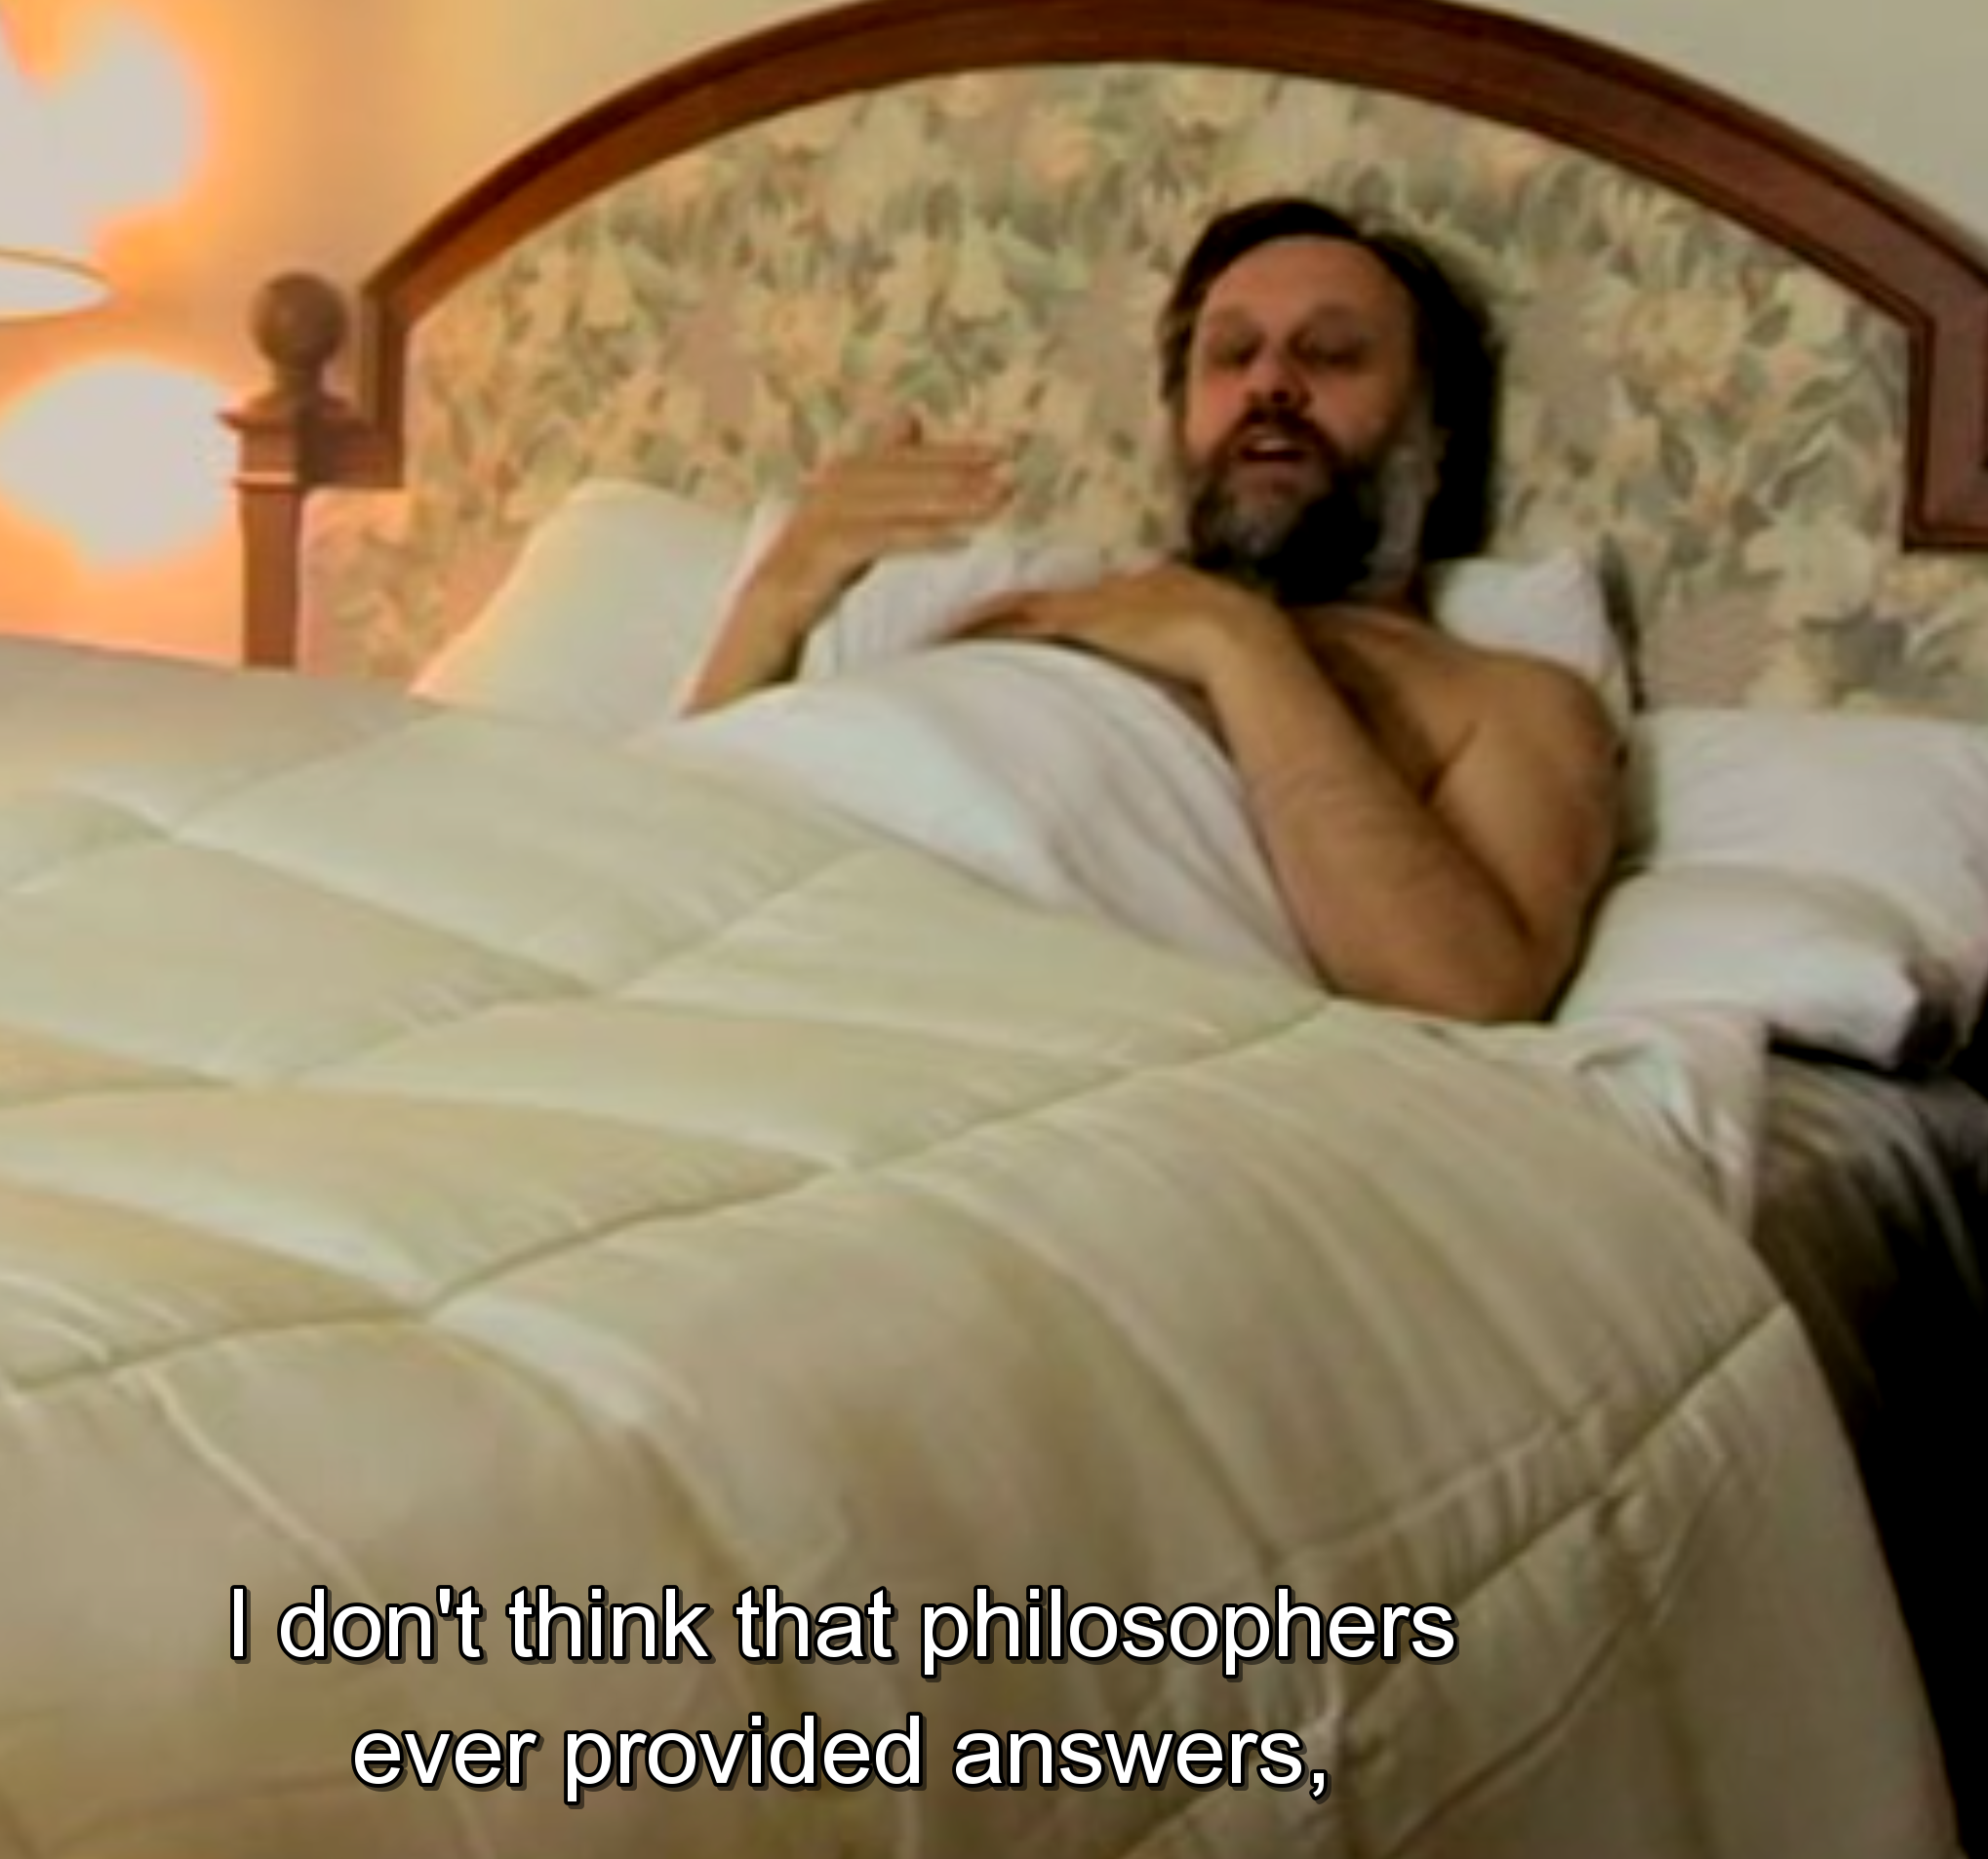
\includegraphics[width=0.5\textwidth]{images/template.png}
%	\caption{Template Bild}
%	\label{fig:template}
%\end{figure}

\end{document}
